\documentclass[onesided]{article}\usepackage[]{graphicx}\usepackage[]{color}
% maxwidth is the original width if it is less than linewidth
% otherwise use linewidth (to make sure the graphics do not exceed the margin)
\makeatletter
\def\maxwidth{ %
  \ifdim\Gin@nat@width>\linewidth
    \linewidth
  \else
    \Gin@nat@width
  \fi
}
\makeatother

\definecolor{fgcolor}{rgb}{0.345, 0.345, 0.345}
\newcommand{\hlnum}[1]{\textcolor[rgb]{0.686,0.059,0.569}{#1}}%
\newcommand{\hlstr}[1]{\textcolor[rgb]{0.192,0.494,0.8}{#1}}%
\newcommand{\hlcom}[1]{\textcolor[rgb]{0.678,0.584,0.686}{\textit{#1}}}%
\newcommand{\hlopt}[1]{\textcolor[rgb]{0,0,0}{#1}}%
\newcommand{\hlstd}[1]{\textcolor[rgb]{0.345,0.345,0.345}{#1}}%
\newcommand{\hlkwa}[1]{\textcolor[rgb]{0.161,0.373,0.58}{\textbf{#1}}}%
\newcommand{\hlkwb}[1]{\textcolor[rgb]{0.69,0.353,0.396}{#1}}%
\newcommand{\hlkwc}[1]{\textcolor[rgb]{0.333,0.667,0.333}{#1}}%
\newcommand{\hlkwd}[1]{\textcolor[rgb]{0.737,0.353,0.396}{\textbf{#1}}}%
\let\hlipl\hlkwb

\usepackage{framed}
\makeatletter
\newenvironment{kframe}{%
 \def\at@end@of@kframe{}%
 \ifinner\ifhmode%
  \def\at@end@of@kframe{\end{minipage}}%
  \begin{minipage}{\columnwidth}%
 \fi\fi%
 \def\FrameCommand##1{\hskip\@totalleftmargin \hskip-\fboxsep
 \colorbox{shadecolor}{##1}\hskip-\fboxsep
     % There is no \\@totalrightmargin, so:
     \hskip-\linewidth \hskip-\@totalleftmargin \hskip\columnwidth}%
 \MakeFramed {\advance\hsize-\width
   \@totalleftmargin\z@ \linewidth\hsize
   \@setminipage}}%
 {\par\unskip\endMakeFramed%
 \at@end@of@kframe}
\makeatother

\definecolor{shadecolor}{rgb}{.97, .97, .97}
\definecolor{messagecolor}{rgb}{0, 0, 0}
\definecolor{warningcolor}{rgb}{1, 0, 1}
\definecolor{errorcolor}{rgb}{1, 0, 0}
\newenvironment{knitrout}{}{} % an empty environment to be redefined in TeX

\usepackage{alltt}
\usepackage[T1]{fontenc}
\linespread{1.5} % Line spacing - Palatino needs more space between lines
\usepackage{microtype} % Slightly tweak font spacing for aesthetics

\usepackage[hmarginratio=1:1,columnsep=20pt]{geometry} % Document margins
%\usepackage{multicol} % Used for the two-column layout of the document
\usepackage[hang, small,labelfont=bf,up,textfont=it,up]{caption} % Custom captions under/above floats in tables or figures
\usepackage{booktabs} % Horizontal rules in tables
\usepackage{float} % Required for tables and figures in the multi-column environment - they need to be placed in specific locations with the [H] (e.g. \begin{table}[H])

\usepackage{lettrine} % The lettrine is the first enlarged letter at the beginning of the text
\usepackage{paralist} % Used for the compactitem environment which makes bullet points with less space between them

% to ignore texts: good for thank messages and paper submissions.
      % \fbox{\phantom{This text will be invisible too, but a box will be printed arround it.}}

\usepackage{abstract} % Allows abstract customization
\renewcommand{\abstractnamefont}{\normalfont\bfseries} % Set the "Abstract" text to bold
%\renewcommand{\abstracttextfont}{\normalfont\small\itshape} % Set the abstract itself to small italic text

\usepackage[]{titlesec} % Allows customization of titles
\renewcommand\thesection{\Roman{section}} % Roman numerals for the sections
\renewcommand\thesubsection{\Roman{subsection}} % Roman numerals for subsections
\titleformat{\section}[block]{\large\scshape\centering}{\thesection.}{1em}{} % Change the look of the section titles
\titleformat{\subsection}[block]{\large}{\thesubsection.}{1em}{} % Change the look of the section titles

\usepackage{fancybox, fancyvrb, calc}
\usepackage[svgnames]{xcolor}
\usepackage{epigraph}
\usepackage{longtable}
\usepackage{pdflscape}
\usepackage{graphics}
\usepackage{pbox} % \pbox{20cm}{This is the first \\ cell}
\usepackage{amsfonts}
\usepackage{amsmath}
\usepackage{amssymb}
\usepackage{rotating}
\usepackage{paracol}
\usepackage{textcomp}
\usepackage[export]{adjustbox}
\usepackage{afterpage}
\usepackage{filecontents}
\usepackage{color}
\usepackage{latexsym}
\usepackage{lscape}       %\begin{landscape} and \end{landscape}
\usepackage{wasysym}
\usepackage{dashrule}

\usepackage{framed}
\usepackage{tree-dvips}
\usepackage{pgffor}
\usepackage[]{authblk}
\usepackage{setspace}
\usepackage{array}
\usepackage[latin1]{inputenc}
\usepackage{hyperref}     %desactivar para link rojos
\usepackage{graphicx}
\usepackage{dcolumn} % for R tables
\usepackage{multirow} % For multirow in tables
\usepackage{pifont}
\usepackage{listings}




% hypothesis / theorem package begin
\usepackage{amsthm}
\usepackage{thmtools}
\declaretheoremstyle[
spaceabove=6pt, spacebelow=6pt,
headfont=\normalfont\bfseries,
notefont=\mdseries, notebraces={(}{)},
bodyfont=\normalfont,
postheadspace=0.6em,
headpunct=:
]{mystyle}
\declaretheorem[style=mystyle, name=Hypothesis, preheadhook={\renewcommand{\thehyp}{H\textsubscript{\arabic{hyp}}}}]{hyp}

\usepackage{cleveref}
\crefname{hyp}{hypothesis}{hypotheses}
\Crefname{hyp}{Hypothesis}{Hypotheses}
% hypothesis / theorem package end


%----------------------------------------------------------------------------------------
% Other ADDS-ON
%----------------------------------------------------------------------------------------

% independence symbol \independent
\newcommand\independent{\protect\mathpalette{\protect\independenT}{\perp}}
\def\independenT#1#2{\mathrel{\rlap{$#1#2$}\mkern2mu{#1#2}}}







\hypersetup{
    bookmarks=true,         % show bookmarks bar?
    unicode=false,          % non-Latin characters in Acrobat's bookmarks
    pdftoolbar=true,        % show Acrobat's toolbar?
    pdfmenubar=true,        % show Acrobat's menu?
    pdffitwindow=true,     % window fit to page when opened
    pdfstartview={FitH},    % fits the width of the page to the window
    pdftitle={My title},    % title
    pdfauthor={Author},     % author
    pdfsubject={Subject},   % subject of the document
    pdfcreator={Creator},   % creator of the document
    pdfproducer={Producer}, % producer of the document
    pdfkeywords={keyword1} {key2} {key3}, % list of keywords
    pdfnewwindow=true,      % links in new window
    colorlinks=true,       % false: boxed links; true: colored links
    linkcolor=ForestGreen,          % color of internal links (change box color with linkbordercolor)
    citecolor=ForestGreen,        % color of links to bibliography
    filecolor=ForestGreen,      % color of file links
    urlcolor=ForestGreen           % color of external links
}

%\usepackage[nodayofweek,level]{datetime} % to have date within text

\newcommand{\LETT}[3][]{\lettrine[lines=4,loversize=.2,#1]{\smash{#2}}{#3}} % letrine customization



% comments on margin
  % Select what to do with todonotes: 
  % \usepackage[disable]{todonotes} % notes not showed
  \usepackage[draft]{todonotes}   % notes showed
  % usage: \todo{This is a note at margin}

\usepackage{cooltooltips}

%%% bib begin
\usepackage[american]{babel}
\usepackage{csquotes}
\usepackage[backend=biber,style=authoryear,dashed=false,doi=false,isbn=false,url=false,arxiv=false]{biblatex}
%\DeclareLanguageMapping{american}{american-apa}
\addbibresource{/Users/hectorbahamonde/Bibliografia_PoliSci/library.bib} 
\addbibresource{/Users/hectorbahamonde/Bibliografia_PoliSci/Bahamonde_BibTex2013.bib} 

% USAGES
%% use \textcite to cite normal
%% \parencite to cite in parentheses
%% \footcite to cite in footnote
%% the default can be modified in autocite=FOO, footnote, for ex. 
%%% bib end

\usepackage{fancyhdr} % Headers and footers
\pagestyle{fancy} % All pages have headers and footers
\fancyhead{} % Blank out the default header
\fancyfoot{} % Blank out the default footer
\fancyhead[C]{Likelihood e Inferencia} % Custom header text
\fancyfoot[RO,LE]{\thepage} % Custom footer text
\IfFileExists{upquote.sty}{\usepackage{upquote}}{}
\begin{document}
% DOCUMENT ID
%----------------------------------------------------------------------------------------
%	CONTENT
%----------------------------------------------------------------------------------------

%\graphicspath{
%{/Users/hectorbahamonde/RU/Term5/Experiments_Redlawsk/Experiment/Data/}
%}



%%%%%%%%%%%%%%%%%%%%%%%%%%%%%%%%%%%%%%%%%%%%%%
% begin knitr stuff


%%%%%%%%%%%%%%%%%%%%%%%%%%%%%%%%%%%%%%%%%%%%%%





\hspace{-5mm}{\bf Profesor}: H\'ector Bahamonde, PhD.\\
\texttt{e:}\href{mailto:hector.bahamonde@uoh.cl}{\texttt{hector.bahamonde@uoh.cl}}\\
\texttt{w:}\href{http://www.hectorbahamonde.com}{\texttt{www.hectorbahamonde.com}}\\
{\bf Curso}: MLE.\\
\hspace{-5mm}{\bf TA}: Gonzalo Barr\'ia.


\section{Likelihood e Inferencia}

Recuerda que \autoref{lik:model} es el ``axiom likelihood''. Lo que dice que likelihood es ``proporcional'' a la probabilidad \parencite[59]{King1998}. Y donde tambi\'en la constante $k(y)$ asegura que el likelihood es relativo al modelo, y no un absoluto como ocurre en el paradigma de la probabilidad.


\begin{equation} \label{lik:model}
\begin{split}
L(\tilde{\theta}|y) & =  k(y)Pr(y|\tilde{\theta})\\
& \propto Pr(y|\tilde{\theta})
%\theta & = g(X, \beta)
\end{split}
\end{equation}


Ahora, tratemos de estimar nuestro par\'ametro $\beta$ pero usando MLE. Es decir, en vez de estimar $\beta \;=\; (x^{\top}x)^{-1}x^{\top}y$, lo estimaremos usando la \autoref{lik:model} de la siguiente manera:


\begin{equation} \label{lik:beta}
\begin{split}
L(\tilde{\beta}|y) & = k(y)Pr(y|\tilde{\beta})\\
                   & = k(y) \prod_{i=1}^{n} f(y_{i}|\tilde{\beta})\\
                   & \propto \prod_{i=1}^{n} f(y_{i}|\tilde{\beta})\\
                   & = \prod_{i=1}^{n} (2\pi)^{-\frac{1}{2}} \exp\left[ \frac{-(y_{i}-\beta)^{2}}{2} \right]
\end{split}
\end{equation}



Importantemente, \autoref{lik:beta} nos entrega el likelihood relativo de que {\bf el modelo (capturado por $\beta$) produzca los datos $y_{i}$}. Sobre esto, hay que rescatar los siguientes puntos:

\begin{enumerate}
  \item MLE es inverso a la probabilidad: en MLE el modelo es construido, y los datos son ``dados''. 
  \item Para hacer obtener el likelihood (que es simplemente un n\'umero), trabajaremos con el conocido ``log-likelihood function'', que es b\'asicamente sacar el log de \autoref{lik:beta} (tal como lo demuestra \autoref{log:lik:beta}).
  \item Usamos \emph{product operators} ($\prod$) porque necesitamos multiplicar el likelihood de cada $i$ particular (cada fila en la columna $y$). Esto es una consecuencia de que por ejemplo $i_{1}$ es independiente a $i_{2}$ y asi para todos los $i_{n}$.
\end{enumerate}

Veamos ahora el ``log-likelihood function'':


\begin{equation} \label{log:lik:beta}
\begin{split}
L(\tilde{\beta}|y) & = k(y)Pr(y|\tilde{\beta})\\
ln \; L(\tilde{\beta}|y) & = ln \; \bigg\{  k(y)Pr(y|\tilde{\beta}) \bigg\} \\
ln \; L(\tilde{\beta}|y) & = -\frac{1}{2} \sum_{i=1}^{n}(y_{i}-\tilde{\beta})^{2}
\end{split}
\end{equation}

Debido a que el logaritmo de un producto ($k(y)Pr(y|\tilde{\beta})$) es la suma de los logaritmos, y adem\'as de que podemos usar el \emph{Fisher-Neyman Factorization Lemma}, la tercera l\'inea es la forma simplificada del ``log-likelihood function''. Nota que $ln \; L(\tilde{\beta}|y)$ depende de los errores cuadrados, es decir, la distancia entre lo predicho y lo observado, i.e. $(y_{i}-\tilde{\beta})^{2} \;=\; \epsilon^{2}_{i}$.

\paragraph{MLE y OLS} Ve\'amos las diferencias, si es que las hay, entre los m\'etodos de estimaci\'on OLS y MLE.

\begin{knitrout}
\definecolor{shadecolor}{rgb}{0.969, 0.969, 0.969}\color{fgcolor}\begin{kframe}
\begin{alltt}
\hlcom{# cocinemos los datos}
\hlstd{n} \hlkwb{<-} \hlnum{1000}
\hlstd{x1} \hlkwb{<-} \hlkwd{rnorm}\hlstd{(n,} \hlkwc{mean} \hlstd{=} \hlnum{150}\hlstd{,} \hlkwc{sd} \hlstd{=} \hlnum{3}\hlstd{)}
\hlstd{x2} \hlkwb{<-} \hlkwd{rnorm}\hlstd{(n,} \hlkwc{mean} \hlstd{=} \hlnum{100}\hlstd{,} \hlkwc{sd} \hlstd{=} \hlnum{2}\hlstd{)}
\hlstd{e}  \hlkwb{<-} \hlkwd{rnorm}\hlstd{(n,} \hlnum{0}\hlstd{)}
\hlstd{y}  \hlkwb{<-} \hlnum{5} \hlopt{+} \hlnum{2}\hlopt{*}\hlstd{x1} \hlopt{+} \hlnum{3}\hlopt{*}\hlstd{x2} \hlopt{+} \hlstd{e}
\hlcom{# OLS:}
\hlstd{ols} \hlkwb{<-} \hlkwd{lm}\hlstd{(y} \hlopt{~} \hlstd{x1} \hlopt{+} \hlstd{x2)}
\hlcom{# GLS}
\hlstd{mle} \hlkwb{<-} \hlkwd{glm}\hlstd{(y} \hlopt{~} \hlstd{x1} \hlopt{+} \hlstd{x2,} \hlkwc{family}\hlstd{=gaussian)}
\hlcom{# Tabla}
\hlkwd{p_load}\hlstd{(texreg)}
\hlkwd{screenreg}\hlstd{(}\hlkwc{l} \hlstd{=} \hlkwd{list}\hlstd{(ols, mle),} \hlkwc{custom.model.names}\hlstd{=}\hlkwd{c}\hlstd{(}\hlstr{"OLS"}\hlstd{,} \hlstr{"MLE"}\hlstd{))}
\end{alltt}
\begin{verbatim}
## 
## =========================================
##                 OLS          MLE         
## -----------------------------------------
## (Intercept)        2.91          2.91    
##                   (2.17)        (2.17)   
## x1                 2.01 ***      2.01 ***
##                   (0.01)        (0.01)   
## x2                 3.01 ***      3.01 ***
##                   (0.02)        (0.02)   
## -----------------------------------------
## R^2                0.99                  
## Adj. R^2           0.99                  
## Num. obs.       1000          1000       
## AIC                           2861.06    
## BIC                           2880.69    
## Log Likelihood               -1426.53    
## Deviance                      1015.30    
## =========================================
## *** p < 0.001; ** p < 0.01; * p < 0.05
\end{verbatim}
\end{kframe}
\end{knitrout}

Como te dar\'as cuenta, ambos m\'etodos dan exactamente los mismos resultados. Es m\'as, la \'ultima l\'inea de la \autoref{log:lik:beta} muestra que el log-likelihood $ln \; L(\tilde{\beta}|y)$ es completamente una funci\'on de $y$. Hasta el momento, nada ha cambiado desde OLS. Bajo ese paradigma, nos enfoc\'abamos en estimar $\beta$, que no es nada m\'as que el valor esperado de una variable mantenida en su \emph{promedio}. En MLE, es bastante parecido. De hecho, \textcite[68]{King1998} explica que ``the maximum likelihood estimator for $\beta$ [...] also has a familiar analytical solution: $\beta \;=\; (x^{\top}x)^{-1}x^{\top}y$''. En vez de $\beta$, en MLE nos concentramos en $\pi$ que tambi\'en es el valor esperado. Sin embargo, cambiamos el modo de leer lo que significa ese valor esperado. Como dice \textcite[66-67]{King1998}, los estimadores MLE tienen ``the highest relative likelihood of having generated the data we observed''.

\paragraph{Por qu\'e usar otro m\'etodo entonces?} En este caso, nosotros sabemos (porque as\'i lo hemos construido), que \texttt{e} tiene promedio 0 (\texttt{e  <- rnorm(n, 0)}). Ya sabemos que este es un ``population parameter'' y que nunca llegaremos a saber si es el promedio es cero ($E(e)\;=\;0$ es un supuesto). Entonces, \emph{por qu\'e usar otro m\'etodo entonces?} Aunque no sabemos si los supuestos se cumplen en la regresi\'on lineal, \emph{s\'i sabemos} que estos supuestos {\bf no se cumplen} en modelos cuyas variables dependientes binarias o categoricas.

\paragraph{C\'omo se ve el log-likelihood?} 

\begin{knitrout}
\definecolor{shadecolor}{rgb}{0.969, 0.969, 0.969}\color{fgcolor}\begin{kframe}
\begin{alltt}
\hlcom{# cocinemos los datos}
\hlstd{n} \hlkwb{<-} \hlnum{1000} \hlcom{# sample size es 1000}
\hlstd{ym} \hlkwb{=} \hlnum{3} \hlcom{# promedio de y es 3.}
\hlcom{# Funcion para encontrar el LL}
\hlstd{pi}\hlkwb{=}\hlkwd{c}\hlstd{(}\hlnum{1}\hlopt{:}\hlnum{100}\hlstd{)}\hlopt{/}\hlnum{100}
\hlstd{logl}\hlkwb{=}\hlkwa{function}\hlstd{(}\hlkwc{pi}\hlstd{) n}\hlopt{*}\hlstd{(ym}\hlopt{*}\hlkwd{log}\hlstd{(}\hlnum{1}\hlopt{-}\hlstd{pi)}\hlopt{+}\hlkwd{log}\hlstd{(pi))}
\hlstd{score}\hlkwb{=}\hlkwa{function}\hlstd{(}\hlkwc{pi}\hlstd{) n}\hlopt{*}\hlstd{(}\hlnum{1}\hlopt{/}\hlstd{pi}\hlopt{-}\hlstd{ym}\hlopt{/}\hlstd{(}\hlnum{1}\hlopt{-}\hlstd{pi))}
\hlstd{logl1}\hlkwb{=}\hlstd{n}\hlopt{*}\hlstd{(ym}\hlopt{*}\hlkwd{log}\hlstd{(}\hlnum{1}\hlopt{-}\hlstd{pi)}\hlopt{+}\hlkwd{log}\hlstd{(pi))}
\hlstd{score1}\hlkwb{=}\hlstd{n}\hlopt{*}\hlstd{(}\hlnum{1}\hlopt{/}\hlstd{pi}\hlopt{-}\hlstd{ym}\hlopt{/}\hlstd{(}\hlnum{1}\hlopt{-}\hlstd{pi))}
\end{alltt}
\end{kframe}
\end{knitrout}

Grafiquemos.

\begin{knitrout}
\definecolor{shadecolor}{rgb}{0.969, 0.969, 0.969}\color{fgcolor}\begin{kframe}
\begin{alltt}
\hlcom{# Grafico}
\hlkwd{plot}\hlstd{(logl,} \hlkwc{col}\hlstd{=}\hlstr{"red"}\hlstd{,}\hlkwc{xlab}\hlstd{=}\hlstr{"pi"}\hlstd{,}\hlkwc{ylab}\hlstd{=}\hlstr{"logl(pi)"}\hlstd{)}
\hlkwd{points}\hlstd{(pi[score1}\hlopt{==}\hlnum{0}\hlstd{],logl1[pi}\hlopt{==}\hlstd{pi[score1}\hlopt{==}\hlnum{0}\hlstd{]],}\hlkwc{pch}\hlstd{=}\hlnum{2}\hlstd{,}\hlkwc{col}\hlstd{=}\hlstr{"red"}\hlstd{,}\hlkwc{cex}\hlstd{=}\hlnum{0.6}\hlstd{)}
\hlkwd{title}\hlstd{(}\hlstr{"log-likelihood function"}\hlstd{)}
\end{alltt}
\end{kframe}

{\centering 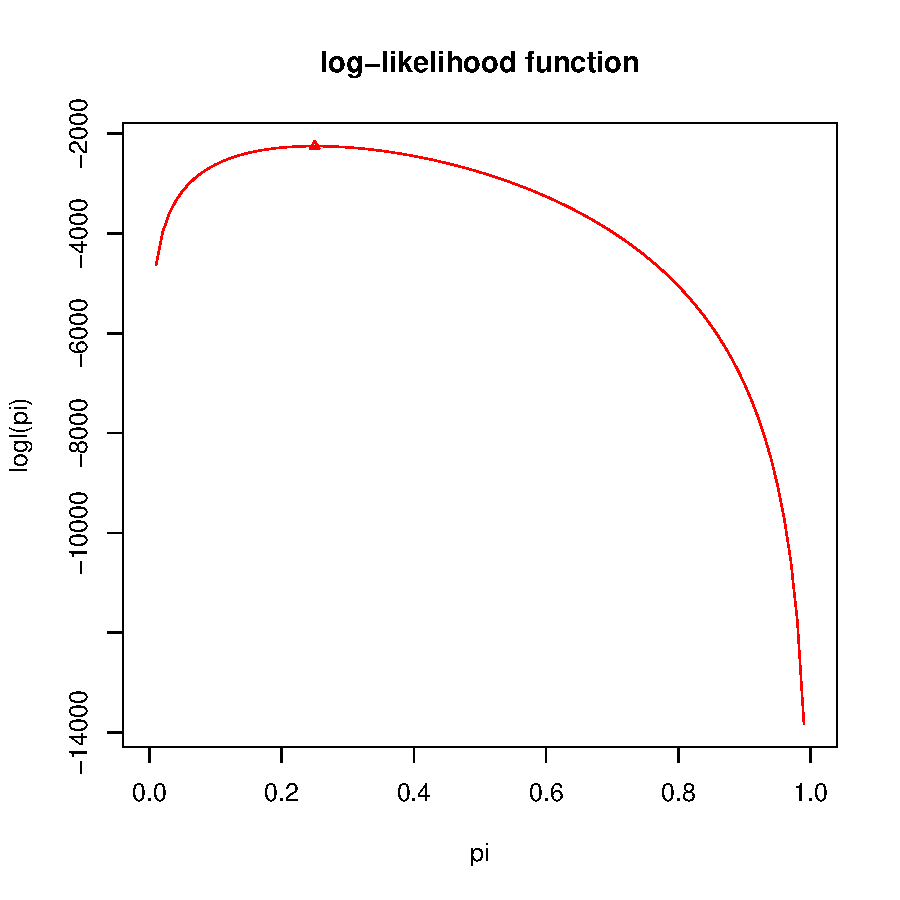
\includegraphics[width=\maxwidth]{figure/ll:p-1} 

}



\end{knitrout}

Como ver\'as, cuando $E(y) \;=\; \pi  \;=\; 3$, el {\bf log-likelihood}, es decir, {\bf el valor que maximiza la posibilidad de que la distribucion de $y$ tenga un promedio 3} es $ln \; L(\hat\theta|y)$ = $-2249.3$ (f\'ijate que reemplazamos $\beta$ por $\hat\theta$ para volver a nuestra notaci\'on MLE). Ve\'amos:

\begin{knitrout}
\definecolor{shadecolor}{rgb}{0.969, 0.969, 0.969}\color{fgcolor}\begin{kframe}
\begin{alltt}
\hlkwd{round}\hlstd{(}\hlkwd{max}\hlstd{(logl1),}\hlnum{1}\hlstd{)}
\end{alltt}
\begin{verbatim}
## [1] -2249.3
\end{verbatim}
\end{kframe}
\end{knitrout}

Al margen de los c\'odigos de \texttt{R}, vemos claramente que $-2249.3$ es el log-likelihood, i.e. el valor que hace que $y$ tenga promedio $3$. \emph{C\'omo se calcula el log-likelihood?}

\section{M\'etodos Anal\'iticos}

\begin{enumerate}
	\item Calcular la derivada de la funci\'on log-likelihood con respecto al vector de par\'ametros  $\tilde\theta$. 
	\item Setear la derivada a 0, y substituir cada elemento de $\tilde\theta$ con $\hat\theta$.
	\item Si es posible, resolver por $\hat\theta$.
	\item Tomar la segunda derivada de la funci\'on log-likelihood. Si es negativa, $\tilde\theta$ es el maximum likelihood estimator. 
\end{enumerate}

Este procedimiento asegura que caigamos en el {\color{red}global maxima} y no en el {\color{blue}local maxima}.

\begin{knitrout}
\definecolor{shadecolor}{rgb}{0.969, 0.969, 0.969}\color{fgcolor}\begin{kframe}
\begin{alltt}
\hlkwd{p_load}\hlstd{(ggplot2,ggpmisc)}
\hlstd{pi} \hlkwb{<-} \hlkwd{seq}\hlstd{(}\hlopt{-}\hlnum{5}\hlstd{,}\hlnum{5}\hlstd{,}\hlkwc{length}\hlstd{=}\hlnum{10001}\hlstd{)}
\hlstd{log.lik} \hlkwb{<-} \hlstd{(}\hlnum{10}\hlopt{*}\hlstd{((pi}\hlopt{-}\hlnum{1}\hlstd{)}\hlopt{^}\hlnum{2}\hlstd{)}\hlopt{^}\hlstd{(}\hlnum{1}\hlopt{/}\hlnum{3}\hlstd{))}\hlopt{/}\hlstd{(pi}\hlopt{^}\hlnum{2} \hlopt{+} \hlnum{9}\hlstd{)}
\hlstd{df} \hlkwb{<-} \hlkwd{data.frame}\hlstd{(}\hlkwc{pi} \hlstd{= pi,} \hlkwc{log.lik} \hlstd{= log.lik)}
\hlkwd{ggplot}\hlstd{(}\hlkwc{data} \hlstd{= df,} \hlkwd{aes}\hlstd{(}\hlkwc{x} \hlstd{= pi,} \hlkwc{y} \hlstd{= log.lik))} \hlopt{+} \hlkwd{geom_line}\hlstd{()} \hlopt{+} \hlkwd{stat_peaks}\hlstd{(}\hlkwc{col} \hlstd{=} \hlkwd{c}\hlstd{(}\hlstr{"red"}\hlstd{,}\hlstr{"blue"}\hlstd{))}
\end{alltt}
\end{kframe}

{\centering 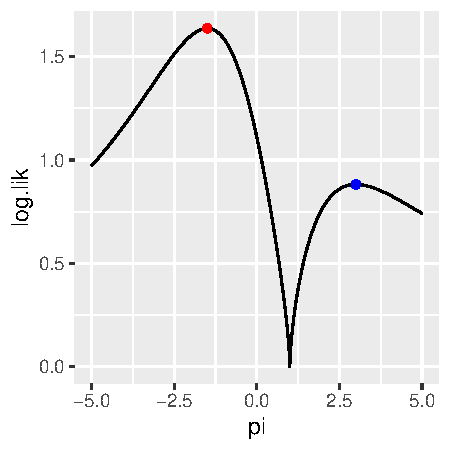
\includegraphics[width=\maxwidth]{figure/local_global_max-1} 

}



\end{knitrout}

\section{M\'etodos Num\'ericos}

Muchas veces resolver por $\hat\theta$ es algebraicamente imposible \parencite[72]{King1998}. Es por esto que este proceso empieza por seleccionar ``valores de partida'' (\emph{starting values}), y a trav\'es de la especificaci\'on de los distintos valores de que puede tomar el parametro $\tilde{\theta}$, vamos viendo si llegamos al global maxima. Esto es justamente lo que se hizo con el ``grid search'' arriba (uno de los dos m\'etodos num\'ericos), y se hace para toda la superficie de la distribuci\'on. El segundo m\'etodo num\'erico es el m\'etodo de ``gradiente''. Este m\'etodo usa la pendiente (slope) para ver cuando la pendiente es cero. En general, nadie usa m\'etodos as\'i. El computador se encarga de maximizar, pero es importante saber qu\'e es lo que est\'a haciendo el programa.


% https://kevintshoemaker.github.io/NRES-746/LAB3.html
% http://people.tamu.edu/~b-wood/Maximum%20Likelihood/RLesson%203.htm
% http://www.maths.usyd.edu.au/u/UG/SM/STAT3022/r/current/Lecture/lecture03_2020JC.html#4
% http://lib.stat.cmu.edu/datasets/sleep
% https://daviddalpiaz.github.io/appliedstats/simple-linear-regression.html#maximum-likelihood-estimation-mle-approach 
% https://www.r-bloggers.com/fitting-a-model-by-maximum-likelihood/
% http://finzi.psych.upenn.edu/R/library/fitdistrplus/html/logLik-plot.html
% https://stackoverflow.com/questions/21671515/how-to-graph-the-log-likelihood-function
% http://www.maths.usyd.edu.au/u/jchan/GLM/glm16_1_sol.pdf
%\newpage
\paragraph{}
\paragraph{}
\pagenumbering{Roman}
\setcounter{page}{1}
\printbibliography






\end{document}


